% =====================================================================
% 附录 AO 真空与壁处理：从抽速到壁条件（注明出处）
% 数值唯一来源：tools/calc/appAO_calc.py -> tools/calc/appAO_calc.txt（本节凡标出数字的量都由它复算）
% 工作点：V=832.2 m^3、A_wall=489.532 m^2、n_e=1e20 m^-3、T_gas=300 K、
%         P_div=5 Pa、P_vessel=1e-6 Pa、S_pump=100 m^3/s（与附录 AJ/AK 同口径）
% 单位写法：数字与单位一律进数学模式；中文只能进 \text{}，不得进 \mathrm{}
% 三种约定：压强用 Pa（工程口径附 mbar L/s）、抽速用 m^3/s、放气率用 Pa m^3/(s m^2)
% 版权口径：只借鉴结论、公式形式与题型，逐节注明书名/作者/年份/卷期页
% 分工：附录 N 讲壁相互作用与偏滤器物理、附录 AJ 讲加料与排灰的粒子账、
%       本附录讲“机器这一侧”：真空系统怎么定抽速、壁怎么被处理、库存被什么卡住
% =====================================================================

\section{真空是什么单位：密度、吞吐量与流导}
\label{sec:app-ao-units}

真空不是「没有东西」，而是一个\textbf{用粒子数写出来的工作点}。偏滤器要 5 Pa 来把氦灰和杂质带走，真空室本底又要 $10^{-6}$ Pa 来保证不把杂质带进芯部。两个数相差六个数量级，却共用同一套泵。这个换算关系决定了后面所有抽速、放气与漏率的量纲。

由理想气体定律，压强与数密度的关系是

\begin{equation}
n=\frac{P}{k_BT},
\label{eq:app-ao-density}
\end{equation}

取 $T=300$ K、$P=5$ Pa（附录 AJ 的偏滤器口径），得 $n=1.20716\times10^{21}$ m$^{-3}$；本底 $10^{-6}$ Pa 对应 $2.41432\times10^{14}$ m$^{-3}$。整个真空室（$V=832.2$ m$^3$）在 5 Pa 下装着 $1.0046\times10^{24}$ 个粒子。而芯部（$n_e=10^{20}$ m$^{-3}$）只有 $8.322\times10^{22}$ 个。\textbf{边界的粒子数比芯部多一个数量级}，这就是为什么「排灰」是一件工程上比「加热」更重的事。

泵的能力用\textbf{吞吐量}写：

\begin{equation}
Q=PS,
\label{eq:app-ao-throughput}
\end{equation}

$S=100$ m$^3$/s 配 5 Pa，得 $Q=500$ Pa$\cdot$m$^3$/s $=5000$ mbar$\cdot$L/s。换成粒子流：$Q/(k_BT)=1.20716\times10^{23}$ s$^{-1}$（与附录 AJ 的抽气粒子流一致）；外部加料 $2.0591\times10^{21}$ s$^{-1}$ 换算成工程单位是 4598.29 sccm：

\begin{equation}
1\ \text{sccm}=4.47797\times10^{17}\ \text{s}^{-1}.
\label{eq:app-ao-sccm}
\end{equation}

\begin{table}[htbp]
\centering
\caption{附录 AO 用的真空工作点（数字与附录 AJ/AK 同口径）}
\label{tab:app-ao-units}
{\small
\begin{tabular}{p{4.6cm}p{3.4cm}p{6.6cm}}
\toprule
量 & 数值 & 说明 \\
\midrule
偏滤器压强 $P_{\rm div}$ & 5 Pa & 排灰与杂质控制的工作点 \\
本底压强 $P_{\rm vessel}$ & $10^{-6}$ Pa & 避免杂质回流芯部 \\
数密度（5 Pa） & $1.20716\times10^{21}$ m$^{-3}$ & 式 \eqref{eq:app-ao-density} \\
数密度（$10^{-6}$ Pa） & $2.41432\times10^{14}$ m$^{-3}$ & 相差六个数量级 \\
真空室粒子数（5 Pa） & $1.0046\times10^{24}$ & 芯部只有 $8.322\times10^{22}$ \\
吞吐量 $Q=PS$ & 500 Pa$\cdot$m$^3$/s & $=5000$ mbar$\cdot$L/s \\
抽走粒子流 & $1.20716\times10^{23}$ s$^{-1}$ & 附录 AJ 口径 \\
外部加料 & 4598.29 sccm & 只占抽气流的 1.7\% \\
\bottomrule
\end{tabular}}
\end{table}

\begin{tip}{5 Pa 与 $10^{-6}$ Pa 差六个数量级，但它们共用一套泵}{tip-app-ao-units}
偏滤器的高压强区靠低温泵「大吃」，真空室的低压强区靠同一批泵的边角余量维持。所以泵的选型要按\textbf{高压强工况}定，而本底目标却由\textbf{放气}决定（AO.3 节）。
\end{tip}

{\small

\textbf{出处：}真空系统的量与工程口径参照 O'Hanlon《A User's Guide to Vacuum Technology》3rd ed.（2003）第 1--3 章。
聚变装置的工作压强与吞吐量口径参照 ITER Physics Basis（\textit{Nuclear Fusion} \textbf{39}, 1999）第 4 章与 Wesson《Tokamaks》4th ed.（2011）第 4 章。
}

\begin{figure}[htbp]
\centering
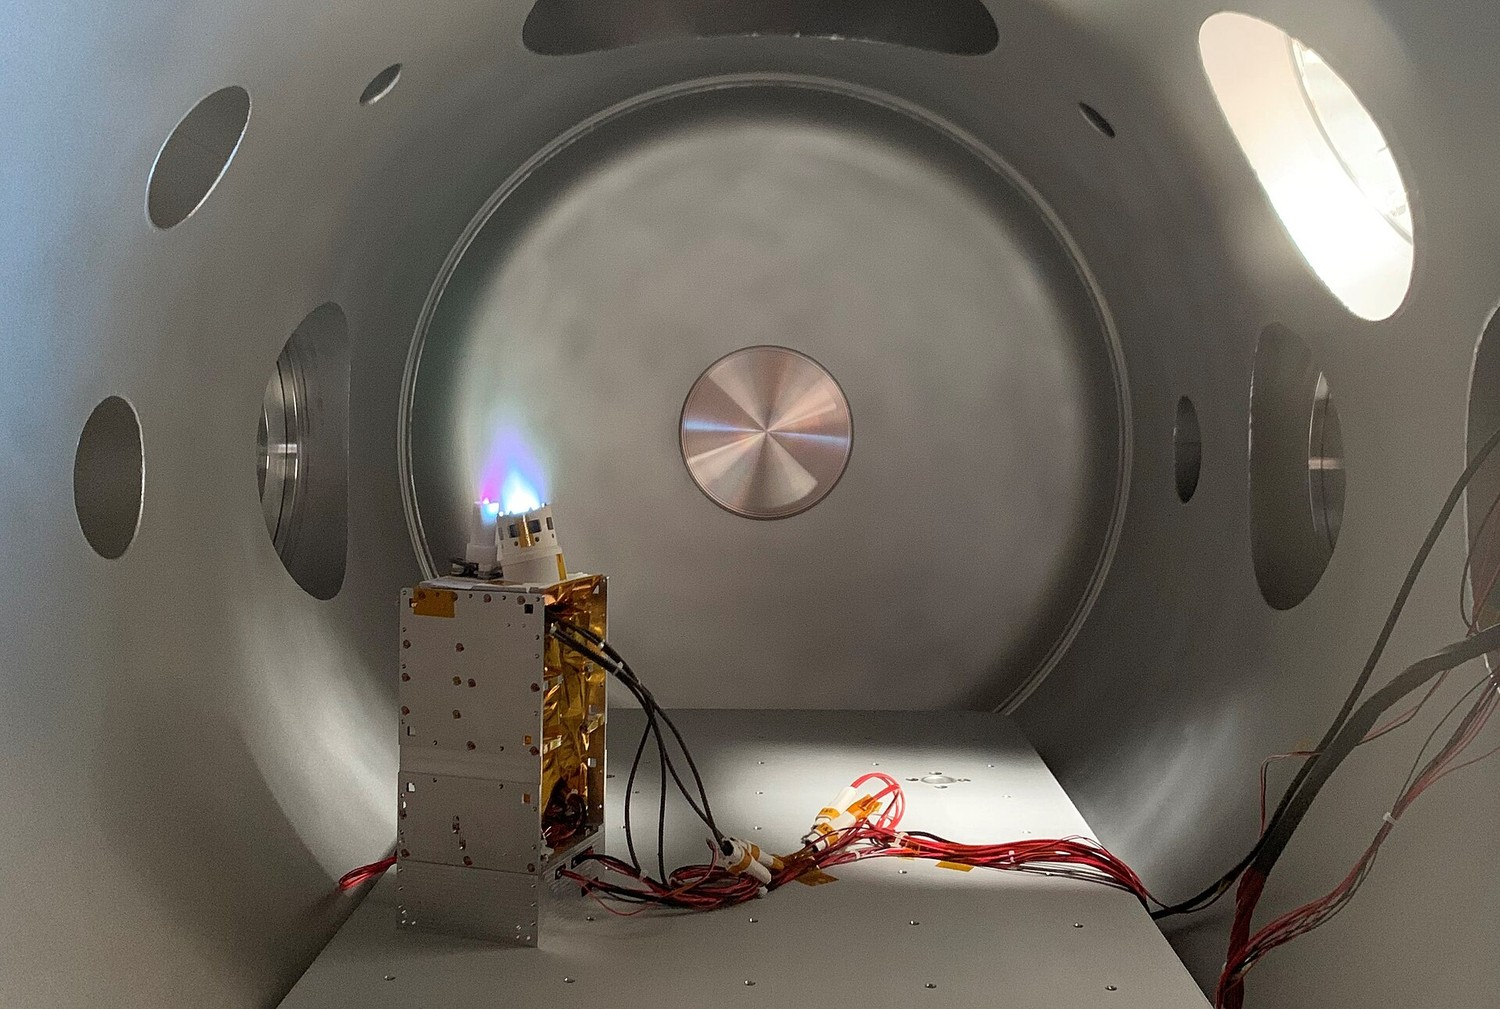
\includegraphics[width=0.72\textwidth]{../figures/thruster_vacuum.jpg}
\caption{真空舱里的放电：抽气与壁条件。推力器在真空舱里点火，舱内压强由抽速与放气共同决定——正是本附录「本底压强是一次除法」与「有效抽速由导管决定」两节所算的场景。}
\label{fig:photo-appao}
\figsource{EXOTRAIL SA，CC BY-SA 4.0（Wikimedia Commons），链接见 figures/CREDITS.md。}
\end{figure}

\begin{figure}[htbp]
\centering
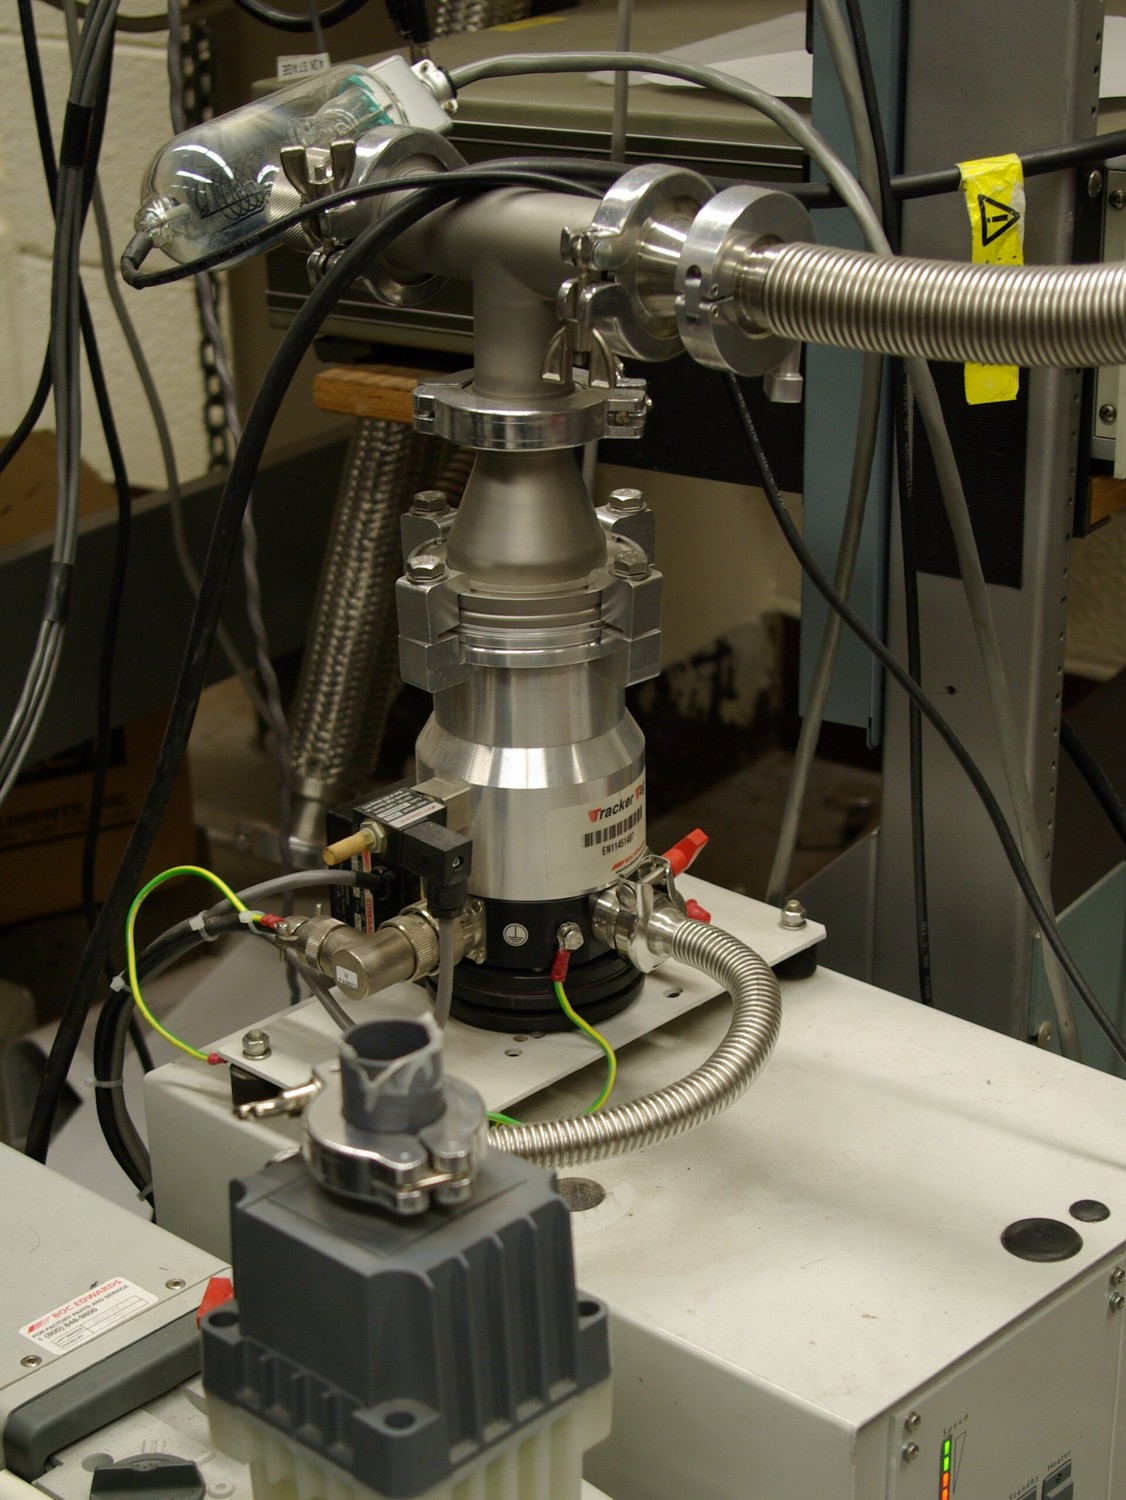
\includegraphics[width=0.67\textwidth]{../figures/turbopump.jpg}
\caption{抽气端的实物：涡轮分子泵。本附录算的有效抽速要乘上一个「泵自己的抽速」：分子泵靠高速转子把气体分子撞向出口，它的抽速只在分子流区间成立——这正是本节把泵与导管放在一起算的原因。}
\label{fig:photo-appao2}
\figsource{Moxfyre，CC BY-SA 4.0（Wikimedia Commons），链接见 figures/CREDITS.md。}
\end{figure}

\begin{figure}[htbp]
\centering
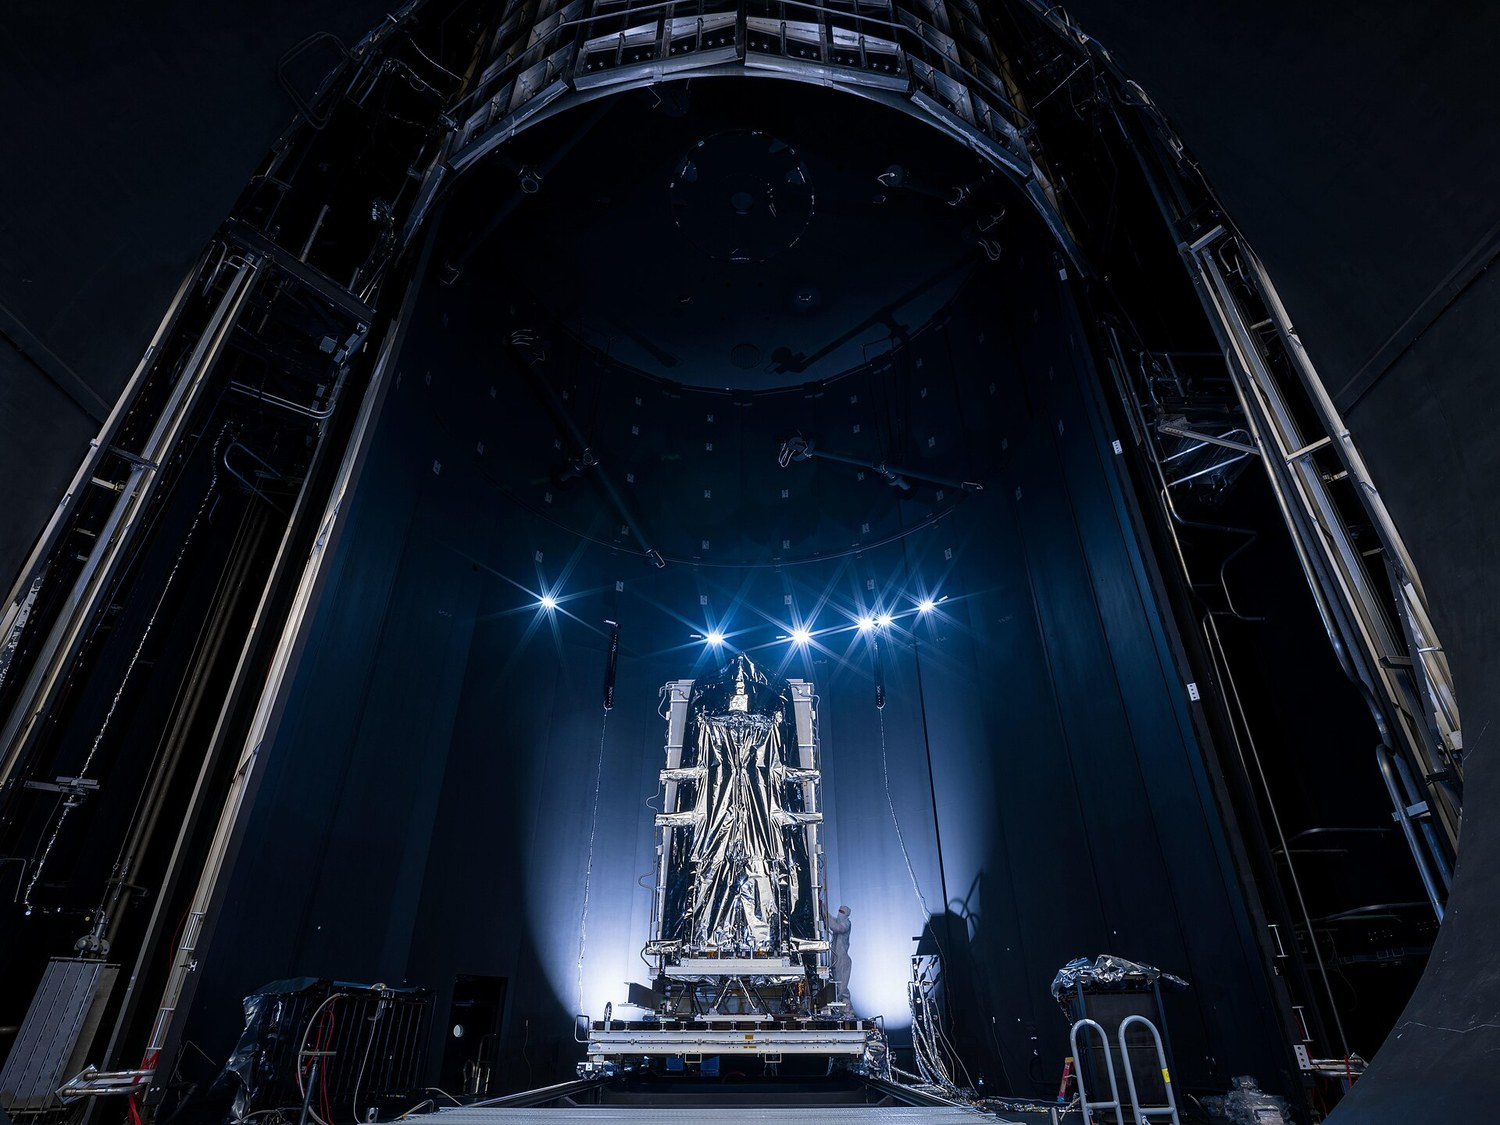
\includegraphics[width=0.72\textwidth]{../figures/ao_chamber_a.jpg}
\caption{真空不是「抽干净」就完事：这样一座热真空室要同时把压强、放气和温度压住。本节的有效抽速、流导与放气率，最终都体现在这类系统级工程的规模上。}
\label{fig:photo-appao3}
\figsource{NASA / Johnson Space Center，Public domain（Wikimedia Commons）}
\end{figure}

\section{抽气：有效抽速由导管决定}
\label{sec:app-ao-pumping}

泵的铭牌抽速和系统的抽速是两件事。粒子要先\textbf{从等离子体走到泵口}，这段路在分子流下就是一段流导：对直径 $d$、长 $L$ 的圆管（20 $^\circ$C 空气），

\begin{equation}
C=12.1\,\frac{d^{3}}{L}\ \ \text{m}^3/\text{s}\quad(d,L\ \text{以 m 计}),
\label{eq:app-ao-conductance}
\end{equation}

直径 1 m、长 1 m 的短管给出 $C=12.1$ m$^3$/s。泵抽速 $S_p$ 与流导串联，系统的\textbf{有效抽速}是

\begin{equation}
S_{\rm eff}=\frac{S_pC}{S_p+C},
\label{eq:app-ao-seff}
\end{equation}

代入 $S_p=100$ m$^3$/s 得 $S_{\rm eff}=10.7939$ m$^3$/s——\textbf{只拿到铭牌的 10.79\%，损失 9.26446 倍}。要让损失不超过一成，需要 $C\ge 9S_p=900$ m$^3$/s，也就是单管直径要做到 4.20551 m（或并联 74.38 根 1 m 短管）：

\begin{equation}
C\ \ge\ 9S_p\quad\Longrightarrow\quad d\ \ge\ \Big(\frac{9S_pL}{12.1}\Big)^{1/3}.
\label{eq:app-ao-lossless}
\end{equation}

偏滤器的泵因此不是「接在管道末端」，而是\textbf{把低温泵直接集成进盒体}：能省的每一米导管，都要用十倍的抽速去补。

还有一条容易被忽略的差别：低温泵对氦的抽速只有对氘的约 10\%。氦是聚变反应的产物、又必须被排走，于是氦的分压会比氘高约 10 倍。\textbf{排灰的瓶颈往往不是总抽速，而是「抽氦的那部分」}。

\begin{table}[htbp]
\centering
\caption{抽气系统的串联关系（$S_p=100$ m$^3$/s，分子流）}
\label{tab:app-ao-pumping}
{\small
\begin{tabular}{p{4.8cm}p{3.2cm}p{6.6cm}}
\toprule
量 & 数值 & 说明 \\
\midrule
导管流导 $C$（1 m$\times$1 m） & 12.1 m$^3$/s & 式 \eqref{eq:app-ao-conductance} \\
有效抽速 $S_{\rm eff}$ & 10.7939 m$^3$/s & 式 \eqref{eq:app-ao-seff} \\
相对铭牌的份额 & 10.79\% & 损失 9.26446 倍 \\
损失一成所需流导 & 900 m$^3$/s & $C\ge 9S_p$ \\
对应单管直径 & 4.20551 m & 式 \eqref{eq:app-ao-lossless} \\
或并联 1 m 短管 & 74.38 根 & 工程上不可行 $\Rightarrow$ 泵进盒体 \\
低温泵对氦的抽速 & 10 m$^3$/s & 约为氘的 1/10 \\
\bottomrule
\end{tabular}}
\end{table}

\begin{tip}{泵的抽速不是系统的抽速}{tip-app-ao-pumping}
买泵看铭牌，设计看流导。分子流下流导正比于 $d^3/L$：\textbf{直径是三次方，长度是一次方}：把导管做短一倍，比把泵换大一倍划算得多。
\end{tip}

{\small

\textbf{出处：}分子流流导与有效抽速的公式参照 O'Hanlon《A User's Guide to Vacuum Technology》3rd ed.（2003）第 3--4 章。
低温泵对氦与氘的抽速差异参照 ITER Physics Basis（\textit{Nuclear Fusion} \textbf{39}, 1999）第 4 章与 Dolan（编）《Magnetic Fusion Technology》（2013）第 6 章。
}

\section{放气与漏率：本底压强是一次除法}
\label{sec:app-ao-outgassing}

真空室的本底压强不是「抽出来的」，而是\textbf{放出来的气体除以抽速}。不锈钢壁在分子流下的放气率 $q$（单位 Pa$\cdot$m$^3$/(s$\cdot$m$^2$)）乘上壁面积就是总放气量：

\begin{equation}
Q_{\rm out}=qA_{\rm wall},
\label{eq:app-ao-outgas}
\end{equation}

未烘烤的不锈钢取 $q=10^{-5}$、$A_{\rm wall}=489.532$ m$^2$，得 $Q_{\rm out}=4.89532\times10^{-3}$ Pa$\cdot$m$^3$/s；平衡压强

\begin{equation}
P_{\rm base}=\frac{Q_{\rm out}}{S}
\label{eq:app-ao-base}
\end{equation}

只有 $4.89532\times10^{-5}$ Pa，比本底目标 $10^{-6}$ Pa \textbf{差 48.9532 倍}。要抽到 $10^{-6}$ Pa，需要 $S=4895.32$ m$^3$/s，所以必须烘烤。350 $^\circ$C 烘烤把放气率压到 $10^{-8}$，于是

\begin{equation}
\frac{P_{\rm baked}}{P_{\rm unbaked}}=\frac{q_{\rm baked}}{q_{\rm unbaked}}=10^{-3},
\label{eq:app-ao-bake}
\end{equation}

平衡压强变成 $4.89532\times10^{-8}$ Pa，相对目标有余量 20.4277 倍。

漏率是另一笔账，而且它和放气\textbf{不是同一个量}：实测总漏率 $3\times10^{-9}$ Pa$\cdot$m$^3$/s 只占烘烤后放气量的 0.061283\%，贡献的压强是 $3\times10^{-11}$ Pa。氦检漏的灵敏度 $10^{-11}$ Pa$\cdot$m$^3$/s 相对实测漏率有 300 倍余量，而允许上限 $10^{-8}$ Pa$\cdot$m$^3$/s 相对实测值也只有 3.33333 倍——\textbf{漏率的余量比放气的余量紧得多}，所以检漏要留到烘烤之后再做，否则放气会把漏信号淹掉。

最后是水。单层水分子在 $A_{\rm wall}$ 上是

\begin{equation}
N_{\rm H_2O}=\sigma_{\rm mono}A_{\rm wall},
\label{eq:app-ao-monolayer}
\end{equation}

$\sigma_{\rm mono}=10^{19}$ m$^{-2}$ 给出 $4.89532\times10^{21}$ 个分子，折合 0.146442 g。听起来很少，但它决定了「抽真空的头几个小时在抽什么」：\textbf{先抽走的是壁上的水，不是室内的气}。

\begin{table}[htbp]
\centering
\caption{放气、本底压强与漏率（$S=100$ m$^3$/s）}
\label{tab:app-ao-outgas}
{\small
\begin{tabular}{p{5.0cm}p{3.6cm}p{6.0cm}}
\toprule
量 & 数值 & 说明 \\
\midrule
未烘烤放气量 & $4.89532\times10^{-3}$ Pa$\cdot$m$^3$/s & $q=10^{-5}$ \\
未烘烤平衡压强 & $4.89532\times10^{-5}$ Pa & 差目标 48.9532 倍 \\
抽到目标所需抽速 & 4895.32 m$^3$/s & 不烘烤则不可能 \\
烘烤后放气量 & $4.89532\times10^{-6}$ Pa$\cdot$m$^3$/s & $q=10^{-8}$ \\
烘烤后平衡压强 & $4.89532\times10^{-8}$ Pa & 余量 20.4277 倍 \\
实测漏率 & $3\times10^{-9}$ Pa$\cdot$m$^3$/s & 占放气 0.061283\% \\
漏率贡献压强 & $3\times10^{-11}$ Pa & 比放气小四个数量级 \\
检漏余量 & 300 倍 & 相对 $10^{-11}$ 灵敏度 \\
单层水分子数 & $4.89532\times10^{21}$ & 0.146442 g \\
\bottomrule
\end{tabular}}
\end{table}

\begin{tip}{本底压强是除法，不是抽功}{tip-app-ao-outgassing}
$P=Q/S$ 里的 $Q$ 和 $S$ 是两笔独立的账：把泵换大一倍只能把压强减半，把壁烘一遍能把 $Q$ 降三个数量级。\textbf{先改分子，再改泵。}
\end{tip}

{\small

\textbf{出处：}放气率与烘烤的数据口径参照 O'Hanlon《A User's Guide to Vacuum Technology》3rd ed.（2003）第 8 章。
托卡马克真空室烘烤与检漏规范参照 ITER Physics Basis（\textit{Nuclear Fusion} \textbf{39}, 1999）第 4 章与 Wesson《Tokamaks》4th ed.（2011）第 4 章。
}

\section{烘烤与壁处理：为什么要把壁「洗」干净}
\label{sec:app-ao-conditioning}

「洗壁」是两件不同的事：\textbf{烘烤}赶走水（AO.3），\textbf{壁处理}改变化学。烘烤本身要先付一笔加热功率：以黑体近似估壁面辐射，

\begin{equation}
P_{\rm bake}=\varepsilon\sigma_{\rm SB}A_{\rm wall}\big(T_{\rm bake}^{4}-T_{0}^{4}\big),
\label{eq:app-ao-bakepower}
\end{equation}

$\varepsilon=0.1$、$T_{\rm bake}=623.15$ K（350 $^\circ$C）给出 396081 W；留一倍对流余量取 792162 W，烘 100 h 要 79.2162 GJ。\textbf{烘烤是一笔电网账}，这也是为什么装置宁愿长期维持低温烘烤（$150$--$200$ $^\circ$C）而不反复升温。

壁处理的代表是硼化：在壁上蒸一层硼，把氧的「来源」变成「汇」。膜厚 $t_B$ 对应质量

\begin{equation}
m_B=A_{\rm wall}t_B\rho_B,
\label{eq:app-ao-boron}
\end{equation}

$t_B=100$ nm、$\rho_B=2.34\times10^{3}$ kg/m$^3$ 得 114.55 g 硼，面密度 $1.30347\times10^{22}$ m$^{-2}$，相当于 1303.47 层单原子。\textbf{一百多克硼就够覆盖半个真空室}，壁处理因此便宜而有效。

放电清洗（GDC/ICWC）则用粒子硬砸：以 $10^{22}$ s$^{-1}$ 的通量洗 1 h 是 $3.6\times10^{25}$ 个粒子，相当于 7353.96 层水膜。它清掉的是碳和氧，代价是壁被溅射、并可能把氚从共沉积层里「翻」出来（AO.6）。

\begin{table}[htbp]
\centering
\caption{烘烤与壁处理的工程账}
\label{tab:app-ao-conditioning}
{\small
\begin{tabular}{p{4.8cm}p{3.4cm}p{6.4cm}}
\toprule
量 & 数值 & 说明 \\
\midrule
烘烤辐射功率 & 396081 W & 式 \eqref{eq:app-ao-bakepower} \\
含对流余量 & 792162 W & 取一倍余量 \\
烘 100 h 的能量 & 79.2162 GJ & 电网账 \\
硼化 100 nm 的硼质量 & 114.55 g & 式 \eqref{eq:app-ao-boron} \\
硼膜面密度 & $1.30347\times10^{22}$ m$^{-2}$ & 1303.47 层单原子 \\
放电清洗 1 h 的粒子数 & $3.6\times10^{25}$ & 约 7353.96 层水膜 \\
\bottomrule
\end{tabular}}
\end{table}

\begin{tip}{壁处理不是打扫，是改变化学}{tip-app-ao-conditioning}
硼化不是把壁「擦干净」，而是让氧优先和硼结合；锂壁、硅化也是同一逻辑。\textbf{壁处理的指标不是清洁度，而是再循环系数与杂质来源的平衡}（AO.5）。
\end{tip}

{\small

\textbf{出处：}硼化与放电清洗的物理参照 Winter（\textit{Plasma Physics and Controlled Fusion} \textbf{38}, 1996）与 Wesson《Tokamaks》4th ed.（2011）第 4 章。
壁处理对再循环的影响参照 ITER Physics Basis（\textit{Nuclear Fusion} \textbf{39}, 1999）第 4 章与 Stangeby《The Plasma Boundary of Magnetic Fusion Devices》（2000）第 4 章。
\section{壁条件与再循环：净加料只是零头}
\label{sec:app-ao-recycling}
}

芯部每秒钟损失的粒子数是 $N/\tau_p$：$N=n_eV=8.322\times10^{22}$、$\tau_p=2.5$ s（附录 AJ 口径）给出 $3.3288\times10^{22}$ s$^{-1}$。这些粒子绝大多数\textbf{没有离开装置}，而是打到壁上、又以中性粒子的形式回来：

\begin{equation}
\Phi_{\rm rec}=R\,\frac{N}{\tau_p},
\label{eq:app-ao-recycle}
\end{equation}

再循环系数 $R=0.95$ 给出 $\Phi_{\rm rec}=3.16236\times10^{22}$ s$^{-1}$，是外部加料（$2.0591\times10^{21}$ s$^{-1}$）的 15.358 倍。真正需要「补」的只是没回来的那部分：

\begin{equation}
\Phi_{\rm net}=(1-R)\,\frac{N}{\tau_p},
\label{eq:app-ao-net}
\end{equation}

$\Phi_{\rm net}=1.6644\times10^{21}$ s$^{-1}$，与外部加料之比是 1.23714——两者同量级，差额来自燃烧掉的粒子与壁上的滞留。\textbf{加料系统的作用不是「喂饱等离子体」，而是补上那 5\% 的零头}；反过来，一旦 $R$ 变化 1\%，净流量就变化 20\%。

壁面承受的通量是

\begin{equation}
\Gamma_{\rm wall}=\frac{1}{A_{\rm wall}}\frac{N}{\tau_p},
\label{eq:app-ao-flux}
\end{equation}

代入得 $6.79996\times10^{19}$ m$^{-2}$s$^{-1}$。这个数乘以溅射产额就是侵蚀率：

\begin{equation}
\dot n_{\rm sput}=Y\,\Gamma_{\rm wall},
\label{eq:app-ao-erosion}
\end{equation}

取 $Y=10^{-4}$（低能氘对钨的量级），得 $6.79996\times10^{15}$ m$^{-2}$s$^{-1}$。和壁面单层原子密度 $10^{19}$ m$^{-2}$ 一比：\textbf{每 1470.6 s（约 24.5 分钟）就能把一整层壁原子打掉一遍}。这不是「几十年才坏」的问题，而是「必须让侵蚀区与再沉积区配对」的问题。偏滤器靶板要厚、要能换，第一壁要选择低溅射材料。

\begin{table}[htbp]
\centering
\caption{壁上的粒子账（$N=8.322\times10^{22}$、$\tau_p=2.5$ s、$R=0.95$）}
\label{tab:app-ao-recycling}
{\small
\begin{tabular}{p{4.8cm}p{3.6cm}p{6.2cm}}
\toprule
量 & 数值 & 说明 \\
\midrule
芯部粒子损失率 & $3.3288\times10^{22}$ s$^{-1}$ & $N/\tau_p$ \\
再循环返回流 & $3.16236\times10^{22}$ s$^{-1}$ & 式 \eqref{eq:app-ao-recycle} \\
净流出 & $1.6644\times10^{21}$ s$^{-1}$ & 式 \eqref{eq:app-ao-net} \\
外部加料/净流出 & 1.23714 & 同量级，差额是燃烧与滞留 \\
再循环/外部加料 & 15.358 & 加料只是零头 \\
壁面通量 & $6.79996\times10^{19}$ m$^{-2}$s$^{-1}$ & 式 \eqref{eq:app-ao-flux} \\
溅射率（$Y=10^{-4}$） & $6.79996\times10^{15}$ m$^{-2}$s$^{-1}$ & 式 \eqref{eq:app-ao-erosion} \\
单层原子被打一遍 & 1470.6 s & 约 24.5 分钟 \\
\bottomrule
\end{tabular}}
\end{table}

\begin{tip}{再循环是乘数}{tip-app-ao-recycling}
$R=0.95$ 意味着壁每秒钟「还回来」95\% 的粒子。它让加料系统显得很小，也让\textbf{任何对 $R$ 的扰动都被放大 20 倍}（分母 $1-R$）。密度控制的稳定性，本质上是壁条件的稳定性。
\end{tip}

{\small

\textbf{出处：}再循环系数与粒子平衡的口径参照 Wesson《Tokamaks》4th ed.（2011）第 4 章与 Stangeby《The Plasma Boundary of Magnetic Fusion Devices》（2000）第 4 章。
溅射产额与侵蚀寿命的量级参照 ITER Physics Basis（\textit{Nuclear Fusion} \textbf{39}, 1999）第 4 章与 Roth 等（\textit{Plasma Physics and Controlled Fusion} \textbf{50}, 2008）的壁侵蚀综述。
}

\section{燃料滞留与氚库存：账在壁上，不在罐里}
\label{sec:app-ao-retention}

氚是放射性的、也是燃料，所以它的\textbf{库存}必须写得出来。滞留有两个通道：一是溶解在壁材料里，二是\textbf{共沉积层}——被溅射下来的碳、硼、钨与氘氚一起重新沉积，把燃料「埋」进一层膜里。后者是可再生装置里最麻烦的一笔。

共沉积层的质量是

\begin{equation}
m_{\rm dep}=A_{\rm dep}t_{\rm dep}\rho_{\rm dep},
\label{eq:app-ao-codep}
\end{equation}

$A_{\rm dep}=100$ m$^2$、$t_{\rm dep}=50$ $\mu$m、$\rho_{\rm dep}=1.8\times10^{3}$ kg/m$^3$ 给出 9000 g。其中碳原子数 $4.51247\times10^{26}$，按 D/C $=0.4$ 得氘氚原子数

\begin{equation}
N_{\rm D}=\Big(\frac{\rm D}{\rm C}\Big)\frac{m_{\rm dep}}{M_{\rm C}u},
\label{eq:app-ao-codepD}
\end{equation}

$=1.80499\times10^{26}$ 个，折合 603.647 g，\textbf{一层 50 $\mu$m 的膜就吃掉 2 kg 库存上限的 30.1823\%}。

另一笔是「每天漏一点」的账：加料氚流 162.72 kg/年（附录 AJ）按 1\% 滞留，每年积 1.6272 kg，

\begin{equation}
t_{\rm limit}=\frac{m_{\rm limit}}{f\,m_{\rm flow}},
\label{eq:app-ao-inventory}
\end{equation}

$m_{\rm limit}=2$ kg、$f=1\%$ 给出 \textbf{1.22911 年}：\textbf{没有清除手段，装置连一年都撑不到库存上限}。去氚（detritiation）与定期壁清洗因此是运行前提，不是环保口号。每清 100 g，一年要清 6.03647 次。

\begin{table}[htbp]
\centering
\caption{氚滞留与库存账（与附录 AJ/AK 同口径）}
\label{tab:app-ao-retention}
{\small
\begin{tabular}{p{4.8cm}p{3.6cm}p{6.2cm}}
\toprule
量 & 数值 & 说明 \\
\midrule
共沉积层质量 & 9000 g & 式 \eqref{eq:app-ao-codep} \\
氘氚原子数 & $1.80499\times10^{26}$ & 式 \eqref{eq:app-ao-codepD} \\
氘氚质量 & 603.647 g & 占库存上限 30.1823\% \\
年滞留量 & 1.6272 kg/年 & 加料流的 1\% \\
达到 2 kg 上限 & 1.22911 年 & 式 \eqref{eq:app-ao-inventory} \\
清除周期（每次 100 g） & 6.03647 次/年 & 运行前提 \\
\bottomrule
\end{tabular}}
\end{table}

\begin{tip}{氚库存的瓶颈在壁上}{tip-app-ao-retention}
燃料罐里的氚是「账面库存」，壁上的氚是「真实库存」。\textbf{共沉积层既存氚、又挡住清除}——它把「库存上限」变成了「清洗频率」的设计约束。
\end{tip}

{\small

\textbf{出处：}共沉积与氚滞留的物理参照 Federici 等（\textit{Nuclear Fusion} \textbf{41}, 2001）与 Roth 等（\textit{Plasma Physics and Controlled Fusion} \textbf{50}, 2008）。
库存与去氚的运行约束参照 ITER Physics Basis（\textit{Nuclear Fusion} \textbf{39}, 1999）第 4 章与 Dolan（编）《Magnetic Fusion Technology》（2013）第 6 章。
\section{估算练习}
\label{sec:app-ao-problems}
}

\begin{enumerate}
\item \textbf{练习 1（抽速加倍）}把抽速从 100 m$^3$/s 提到 200 m$^3$/s，烘烤后的平衡压强是多少？相对 $10^{-6}$ Pa 的本底目标还剩多少余量？
\item \textbf{练习 2（导管变细）}把导管直径从 1 m 改成 0.5 m（长度仍 1 m），流导与有效抽速各是多少？相对 AO.2 节的 1 m 管差多少倍？
\item \textbf{练习 3（漏率）}一个 $10^{-8}$ Pa$\cdot$m$^3$/s 的漏点，在 $S=100$ m$^3$/s 下贡献多少本底压强？占 $10^{-6}$ Pa 目标的份额是多少？
\item \textbf{练习 4（硼化加倍）}把硼化膜厚从 100 nm 加到 200 nm，需要多少硼？相当于多少层单原子？
\item \textbf{练习 5（再循环降低）}若壁条件变差使 $R$ 从 0.95 降到 0.9，净流出粒子流与「外部加料/净流出」之比各变成多少？
\item \textbf{练习 6（共沉积面积加倍）}把共沉积面积从 100 m$^2$ 改成 200 m$^2$（厚度不变），氘氚质量是多少？占 2 kg 库存上限多少？
\end{enumerate}

\textbf{解答 1}$P=Q_{\rm out}/S$：放气量 $4.89532\times10^{-6}$ Pa$\cdot$m$^3$/s 除以 200 m$^3$/s，得 $2.44766\times10^{-8}$ Pa，比原来（100 m$^3$/s）正好小一半，相对 $10^{-6}$ Pa 的余量从 20.4277 倍提到 40.8553 倍。\textbf{结论：抽速只做除法，放气率才做数量级。}

\textbf{解答 2}$C=12.1\,d^3/L=12.1\times0.5^3/1=1.5125$ m$^3$/s（直径减半，流导掉到 1/8）；有效抽速 $S_{\rm eff}=100\times1.5125/(100+1.5125)=1.48996$ m$^3$/s，比 1 m 管的 10.7939 m$^3$/s 差 7.24442 倍。\textbf{这就是 $d^3$ 的代价。}

\textbf{解答 3}$P=Q_{\rm leak}/S=10^{-8}/100=10^{-10}$ Pa，占 $10^{-6}$ Pa 目标的 0.0001（$0.01\%$）。\textbf{漏率一般不是本底压强的限制因素，放气才是}。所以检漏的指标要按「能看见多小的漏」定，而不是按「漏会不会抬高本底」定。

\textbf{解答 4}$m_B=A_{\rm wall}t_B\rho_B=489.532\times200\times10^{-9}\times2.34\times10^{3}=229.101$ g，面密度 $2.60694\times10^{22}$ m$^{-2}$，相当于 2606.94 层单原子。\textbf{硼的用量很便宜，膜厚主要由「能撑多久」决定。}

\textbf{解答 5}$\Phi_{\rm net}=(1-0.9)\times3.3288\times10^{22}=3.3288\times10^{21}$ s$^{-1}$（净流出翻倍）；外部加料与净流出之比降到 0.618571：\textbf{同一个加料系统在 $R=0.9$ 时只能补上六成净损失}，密度会掉下来：这正是「壁条件决定密度控制」的定量版本。

\textbf{解答 6}质量与面积成正比：$603.647\times2=1207.29$ g，占 2 kg 上限的 0.603647（$60.3647\%$）。\textbf{共沉积面积翻倍，库存上限就用掉六成}。所以「把沉积限制在可清除的小区域」本身就是库存控制策略。


\section{来源、分级与版权说明}
\label{sec:app-ao-source}

\begingroup\small
这一篇只讲\textbf{「机器这一侧」的三件事}：真空系统怎么把压强写出来（AO.1--AO.3）、壁怎么被处理与再循环怎么被放大（AO.4--AO.5）、氚库存被什么卡住（AO.6）。

\begin{table}[htbp]
\centering
\caption{本附录的借鉴来源与处理方式}
\label{tab:app-ao-source}
{\small
\begin{tabular}{p{3.4cm}p{4.6cm}p{6.4cm}}
\toprule
借鉴内容 & 来源 & 本书的处理 \\
\midrule
真空量与流导公式 & O'Hanlon《A User's Guide to Vacuum Technology》3rd ed.（2003）第 1--4、8 章 & 重写推导，只保留结论与可复算系数 \\
放气率与烘烤数据 & 同上，第 8 章 & 取量级作声明输入，数值全部由 \texttt{appAO\_calc.py} 复算 \\
托卡马克工作压强与吞吐量 & ITER Physics Basis（\textit{Nuclear Fusion} \textbf{39}, 1999）第 4 章 & 只取口径（5 Pa / $10^{-6}$ Pa / 100 m$^3$/s） \\
壁处理与再循环 & Wesson《Tokamaks》4th ed.（2011）第 4 章；Stangeby（2000）第 4 章 & 改写为「净流量 = (1-R)」的账 \\
硼化与放电清洗 & Winter（\textit{PPCF} \textbf{38}, 1996） & 只引用原理结论，不复制工艺配方 \\
溅射与侵蚀寿命 & Roth 等（\textit{PPCF} \textbf{50}, 2008） & 只取产额量级，题型自拟 \\
共沉积与氚滞留 & Federici 等（\textit{Nuclear Fusion} \textbf{41}, 2001） & 只取 D/C 比与层厚量级 \\
库存与去氚约束 & Dolan（编）《Magnetic Fusion Technology》（2013）第 6 章 & 与附录 Z/AJ/AK 同口径，改写为 1.22911 年这笔账 \\
\bottomrule
\end{tabular}}
\end{table}

\textbf{不复制什么：}

\begin{itemize}
\item 不复制文献中的真空系统总布置图、泵组配置与管路走向；
\item 不复制各文献使用的符号体系（本书统一用 $q$、$Q$、$S$、$C$、$R$、$f$）；
\item 不复制任何教科书或论文中的习题原题（本附录六道题均为自拟，数值全部可复算）；
\item 不复制硼化/放电清洗的工艺配方、气体配比与时间-温度曲线；
\item 不复制文献对氚滞留数据的逐年统计表。
\end{itemize}

\begin{tip}{本附录没有涵盖什么}{tip-app-ao-honest}
这一篇不设计真空系统、不展开泵的选型与管路布置、也不展开具体的去氚工艺参数。它只做一件事：把「压强、抽速、放气、漏率、再循环、库存」这六个量之间的\textbf{除法与乘法关系}写清楚，其余留给专门的工程文献。
\end{tip}

本附录所有标出的数字都由 \texttt{tools/\allowbreak{}calc/\allowbreak{}appAO\_calc.py} 复算；工作点与附录 AJ/AK 完全一致（$V=832.2$ m$^3$、$A_{\rm wall}=489.532$ m$^2$、$n_e=10^{20}$ m$^{-3}$、$P_{\rm div}=5$ Pa、$S=100$ m$^3$/s）。
\endgroup
